\begin{frame}
    \frametitle{Introduzione}
    \addtocounter{nframe}{1}
    
    %\begin{center}
    %    
\includegraphics[width=.2\textwidth]{../imgs/tei-r.pdf}
    %\end{center}

    \begin{block}{Cos'è la TEI}
        la TEI - \textit{acronimo di Text Encoding Initiative} - rappresenta un punto di riferimento per tutte le iniziative il cui scopo principale è quello di digitalizzare risorse testuali in ambito umanistico per fini di ricerca e di conservazione.
    \end{block}
    
\end{frame}

%%
<add> una o più parole aggiunte nel testo
questa parola è <add place="supralinear">stata</add> aggiunta in un secondo momento
<del> una o più parole cancellate nel testo
questa invece era <del rend="overstrike">era</del>
 di troppo e l’ho cancellata
<gap/> parte di testo omessa, mancante o illeggibile
questa <gap reason="illegible" extent="6" unit="chars"/> è illeggibile (forse “parola”?)

%%
<damage> testo danneggiato nel documento originale
   
per qualche goccia d’acqua questa parola si è
   <damage agent="water">scolorita</damage> molto

   <unclear> parte di testo interpretabile con difficoltà
<unclear reason="faded">questa</unclear> si legge
   ancora ma con difficoltà

   <supplied> testo inserito dal curatore perché illeggibile nell’originale o assente (fa parte del modulo transcr)
qui <supplied>mancava qualcosa</supplied> nel testo

è possibile combinare questi elementi (compreso <gap/>)

%%
Dal Vercelli Book: manoscritto in inglese antico, dialetto tardo sassone occidentale, X secolo ca.
   %\begin{center}
    %    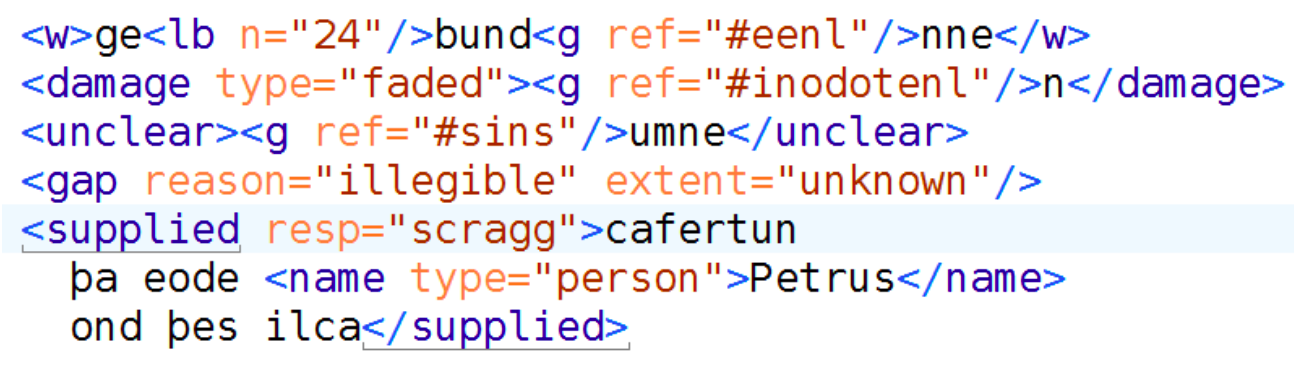
\includegraphics[width=.9\textwidth]{/imgs/vercelli.png}
    %\end{center}

%%
- può succedere che una parola non sia semplicemente cancellata, ma che sia anche sostituita da un altro termine
- in questo caso è possibile usare l’elemento <subst> per collegare la sequenza cancellazione → nuovo testo

%%
questa parola è stata <subst>
<del rend="overstrike">scritta</del>
<add place="supralinear">aggiunta</add>
<subst> in un secondo momento

anche a livello della singola lettera
<subst><del rend="overtype">t<del><add>T</add></subst>i scrivo una
   mail domani mattina

   <subst> fa parte del modulo transcr, per ulteriori informazioni (@seq) v. http://www.tei- c.org/release/doc/tei-p5-doc/en/html/PH.html\#PHSU

%%
Attributi e valori consigliati

- <add> 
place inline, supralinear, margin, etc.
hand author, scribe1, scribe2

- <del> 
rend overstrike, subpunct, overtype, dotted
hand author, scribe1, scribe2

- <gap>
reason illegible, cancelled, irrelevant, missing, omissis, censored 
hand editor
agent water, smoke, hole, missing page
extent chars, words, cm

- <unclear> 
reason parterased, ink blot 
hand author, scribe1, scribe2
agent water, smoke, ink

%%
Correzioni e normalizzazioni

 <sic> parola o frase ritenuta errata, ma riportata “com’è”
questa parola è <sic>statta</sic> sbagliata

<corr> correzione di una parola o frase errata
questa parola è <corr>stata</corr> corretta in un
 secondo momento

<orig> parola o frase ritenuta “non standard” 
Allora, mi dici <orig>’ndo</orig> vai?

<reg> parola o frase normalizzata (regularised) Allora, mi dici <reg>dove</reg> vai?

%%

Abbreviazioni ed espansioni 1 <abbr> parola abbreviata, brevigrafo
 chiedi al <abbr>dott.</abbr> Rossi
 in nomine Patris <abbr>7</abbr> Filii
 <abbr>7</abbr> Spiritus Sancti

<expan> espansione di un’abbreviazione chiedi al <expan>dottor</expan> Rossi
 in nomine Patris <expan>et</expan> Filii
 <expan>et</expan> Spiritus Sancti

 %%
 
<abbr> usare l’attributo type per specificare il tipo chiedi al <abbr type="titolo">dott.</abbr> Rossi
 in nomine Patris <abbr type="brevigrafo">7</abbr> Filii
 <abbr type="brevigrafo">7</abbr> Spiritus

 %%
disponibili ulteriori elementi aggiungendo il modulo transcr:
<am> lettere o segni di abbreviazione
<ex> lettere aggiunte espandendo un’abbreviazione
 <abbr>sanct<am>u~</am></abbr>
 <expan>sanctu<ex>m</ex></expan>

 %%
 alcuni elementi di intervento editoriale sono perfettamente speculari:
<sic> - <corr> <orig> - <reg> <abbr> - <expan>

%%

la relazione fra le coppie è importante per essere sicuri che ciascun elemento sia collegato all’altro

Nella TEI P5 è stato introdotto un nuovo elemento <choice> che comprende ogni coppia

%%
- <sic> - <corr>
questa parola è <choice>

<sic>statta</sic>
<corr>stata</corr> </choice> scritta sbagliata

- <orig> - <reg>
Allora, mi dici <choice><orig>’ndo</orig> <reg>dove</reg></choice> vai?

- <abbr> - <expan>
chiedi al <choice><abbr>dott.</abbr> <expan>dott<ex>or</ex></expan></choice> Rossi

%%
Attributi @resp e @cert
- per <add> e <del> abbiamo l’attributo @hand per specificare, se necessario, l’autore della modifica all’originale
- per qualche intervento editoriale, invece, potrebbe essere importante specificare il responsabile (in particolare per l’elemento <supplied>!) e il grado di certezza
- per fare questo si usano gli attributi @resp e @cert

%%
questa parola è <choice>
<sic>statta</sic>
<corr resp="rrdt">stata</corr> </choice> scritta per errore
- il valore di @resp può rimandare a un <respStmt>: <corr resp="\#rrdt">stata</corr>

%%

Altri elementi utili 1

<gb/> gathering begins: indica l’inizio di un nuovo fascicolo nella trascrizione di un manoscritto

<space> usato per marcare la presenza di spazio significativo (ad esempio spazio lasciato dallo scriba per inserire una iniziale miniata)
normalmente usato come elemento vuoto modulo linking

<pc> punctuation character(s): contiene uno o più caratteri che costituiscono una forma di punteggiatura nel testo

modulo analysis

%% 
- <ab> anonymous block: contenitore di testo simile a un paragrafo ma senza il valore semantico di quest’ultimo
– modulo linking
- <seg> arbitrary segment: usato per marcare qualunque porzione di testo,
usare @type per specificare il contenuto semantico – modulo linking
- <w> word: marca una parola a livello grammaticale, @lemma per indicare il lemma e @lemmaref per stabilire un link con un dizionario online
– modulo analysis
- <c> character: marca un singolo carattere nel testo
– modulo analysis

%% 
Esempio

%%
Esempio

Dal Vercelli Book (inglese antico, dialetto tardo sassone occidentale, X secolo ca.
<del rend="erasure">ff</del>fore wæron
<del rend="dot"><g ref="\#aeligddot"/></del>

%% 
Esempio choice

%% esempi presi con screenshot
